\section{VisualSfM}\label{sec:visualsfm}
%======================================================================================
%
\subsection*{Introdução}

VisualSfM~\cite{wu2011visualsfm} é um \emph{software} baseado em fotogrametria que faz todo o processo de reconstrução 3D de um objeto e que pode ser usado por linha de comando ou então pela interface gráfica, que é ótima, por sinal. É altamente customizável, podemos utilizar o CUDA da NVIDIA, ou OpenGL, especificar a lista de pares para correspondência de imagens, usar detectores de \emph{features} próprios, velocidade da detecção de \emph{features}, da reconstrução densa, dentre outros parâmetros. Ou seja, é um \emph{software} robusto, que pode ser usado em Linux, Windows ou até mesmo Mac.

Além disso, o VisualSfM é capaz de mostrar a matriz de correspondência de \emph{features}, número de \emph{features}, rodar um \emph{Bundle Adjustment} independente, usar um Level 0 no PVMS, alterar a memória de GPU usada na reconstrução, deletar uma reconstrução indesejável ou até mesmo alterar parâmetros.

\subsection*{Procedimento}

Sua linha de reconstrução é parecida com o MVE~\ref{sec:mve}, porém é mais intuitiva. Em sua interface, possui um Log de mensagens e erros que por ventura venham a acontecer e na parte de cima, alguns botões \ref{fig:pipelineVisualSfM}

\begin{figure}[!h]
	\centering

	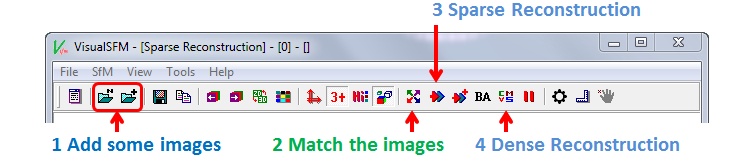
\includegraphics[width=1\linewidth]{figs/pipelinevisualsfm.png}
	\caption{%
	Botões na parte superior da interface gráfica, este seria o \emph{pipeline} padrão de funcionamento do \emph{software}.
	\cite{wu2011visualsfm}
	}\label{fig:pipelineVisualSfM}
\end{figure}

Como demonstrado na imagem \ref{fig:pipelineVisualSfM}, o funcionamento seria da seguinte forma:

\begin{itemize}
\item \textbf{1 - Adicionar algumas imagens.} Este é o primeiro passo, para começar uma reconstrução, primeiro adiciona-se imagens ao \emph{software}, pode ser uma única foto, um conjunto de fotos, incrementar o conjunto já existente ou então abrir um arquivo de extensão .nvm, que é interpretado como uma reconstrução esparsa previamente feita.

\item \textbf{2 - Correspondência de imagens.} Agora, o \emph{software} roda o algoritmo SIFT, realizando todas as correspondências entre os \emph{features}, que já foi discutido anteriormente.

\item \textbf{3 - Reconstrução esparsa.} Neste passo, o VisualSfM roda o algoritmo de reconstrução esparsa (PBA/MCBA)~\cite{wu2011multicore} em todos os \emph{features} descobertos no passo passado. 


PBA/MCBA -- \emph{Multi-Core Bundle Adjustment}\label{pba}

\emph{Bundle} refere-se aos feixes de luz que refletem em cada \emph{feature} 3D e vão para o centro de cada câmera da cena a ser reconstruída. Com isso, o \emph{Bundle Adjustment} é o problema de refinar uma reconstrução visual para produzir estimativas com a visualização de parâmetros (estimativa e/ou calibração de câmeras), juntamente com as estruturas 3D.

Solucionadores de problemas de \emph{Bundle Adjustment}~\cite{bundleAdjustmentSlide} resumem-se em minimizar o erro de reprojeção \ref{fig:bundleAdjustment} entre as posições de imagem dos pontos de imagem observados e previstos, o que é expresso como a soma de quadrados de um grande número de funções não-lineares de valor real. Assim, a minimização é obtida usando algoritmos de mínimos quadrados não-lineares. Destes, Levenberg-Marquardt~\cite{more1978levenberg} provou ser um dos mais bem sucedidos devido à sua facilidade de implementação e ao uso de uma estratégia de amortecimento eficaz que lhe confere a capacidade de convergir rapidamente de uma ampla gama de suposições iniciais. Ao linearizar iterativamente a função a ser minimizada na vizinhança da estimativa atual, o algoritmo de Levenberg-Marquardt envolve a solução de sistemas lineares denominados equações normais. Ao resolver os problemas de minimização que surgem na estrutura do \emph{Bundle Adjustment}, as equações normais tem uma estrutura de bloco esparsa devido à falta de interação entre os parâmetros para diferentes pontos 3D e câmeras. Isso pode ser explorado para obter enormes benefícios computacionais ao empregar uma variante esparsa do algoritmo de Levenberg-Marquardt que aproveita explicitamente o padrão de zeros de equações normais, evitando armazenar e operar em elementos zero.

\begin{figure}[!h]
	\centering
	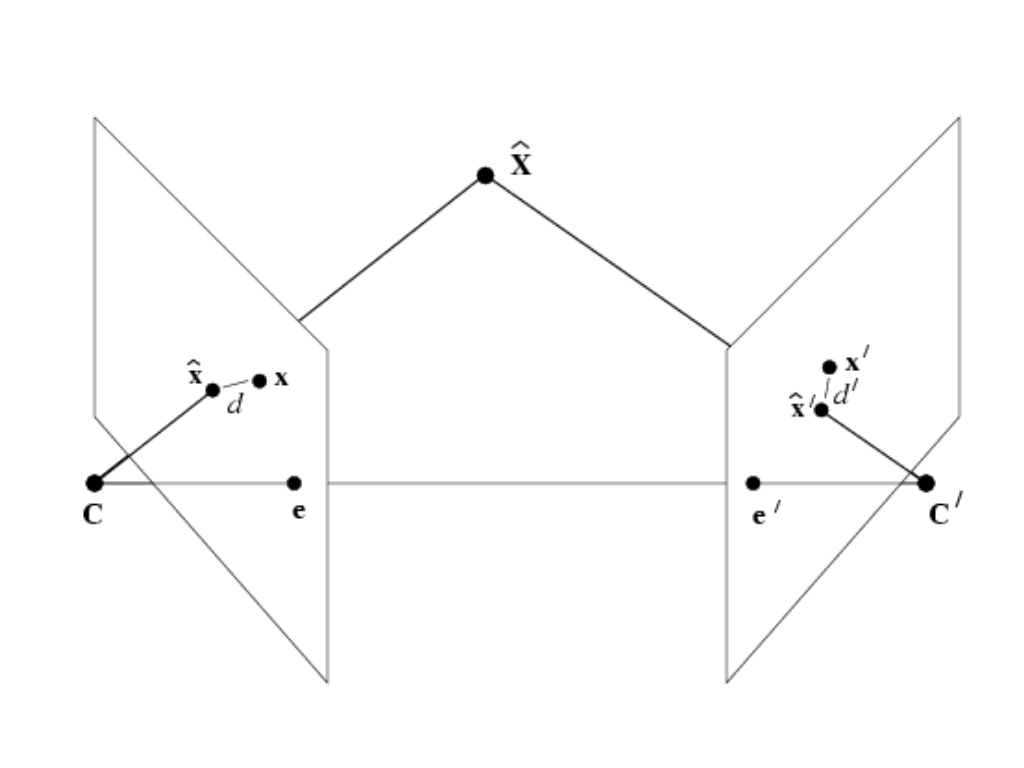
\includegraphics[width=0.5\linewidth]{figs/bundleAdjustment.png}
	\caption{%
	Dado um ponto de um objeto 3D $X^\hat$, sua reprojeção nas câmeras $C$ e $C'$, são, respectivamente, $x$ e $x'$. Esses pontos possuem um erro de reprojeção $d$ e $d'$ e ao utilizar o PBA/MCBA, os pontos $x$ e $x'$ serão reajustados como $x^\hat$ e $x^\hat '$, respectivamente. 
	\cite{3DCompVision2Didier}.
	}\label{fig:bundleAdjustment}
\end{figure}

Neste caso, o PBA/MCBA~\cite{furukawa2009accurate,wu2011multicore} é um algoritmo que utiliza, de forma eficiente, os núcleos do computador, sendo até 10 vezes mais rápido, em CPU e 30 vezes, em GPU, em comparação ao utilizado na conferência ECCV de 2010. É o primeiro sistema publicado, baseado em GPU que escala com maiores problemas de Bundle Adjustments. Isto abriu a porta para resolver problemas ainda maiores. Ele funciona observando o passo inexato de resolução não-linear usando Levenberg Mardquardt, que pode ser implementado sem armazenar nenhuma matriz (Hessiana, complemento de Schur ou Jacobiana) na memória. Para sistemas de núcleo único isso se traduzia em memória de troca por tempo, mas em GPUs, isso leva a um surpreendente ganho, no espaço e no tempo. Outra surpresa é que a aritmética de precisão única, quando combinada com técnicas de normalização adequadas, dá resultados comparáveis aos obtidos por um solucionador de problemas usando aritmética de dupla precisão. Isso resulta em mais espaço e economia de tempo.

Este algoritmo recebe como entrada conjunto de localizações e correspondências de \emph{features} de imagens, o objetivo do \emph{Bundle Adjustment} é encontrar posições de 3 pontos e parâmetros de câmera que minimizem o erro de reprojeção. Esse problema de otimização geralmente é formulado como um problema de mínimos quadrados não-lineares, onde o erro é a norma L2 quadrada da diferença entre a localização da característica observada e a projeção do ponto 3D correspondente no plano da imagem da câmera.

Assumindo que $x$ é um vetor de parâmetros e $f(x) = [f1(x), \dots, f_k(x)]$ é o vetor de erros de projeção de uma reconstrução 3D. O problema de otimização pode ser  formulado como um problema de mínimos quadrados não-linear:

\begin{equation}
x^* = \text{argmin}_x \sum_{i=1}^k || f_i(x)||^2
\end{equation}

O algoritmo de Levenberg-Marquardt (LM) é o mais conhecido para resolução de problemas de mínimos quadrados não-lineares. O LM funciona resolvendo uma série de aproximações lineares regularizadas ao problema não-linear original. Seja $J(x)$ a Jacobiana de $f(x)$, então em cada iteração LM resolve um problema linear de mínimos quadrados da forma:

\begin{equation}
\label{eq:LM}
\delta* = \text{argmin}_\delta || J(x)\delta + f(x) ||^2 + \lambda ||D(x)\delta||^2 
\end{equation}
e, atualiza $x$, da forma:

\begin{algorithm}
\label{LMattX}
\begin{algorithmic}[1]
\State $\text{caso} (||f(x + \delta^*)|| < || f(x) ||)$
\State	$x = x + \delta^*$
\end{algorithmic}
\end{algorithm}

%\begin{algorithmic}[1]
%\BState $\text{caso} (||f(x + \delta^*)|| \le || f(x) ||)$
%\State	$x = x + \delta^*$
%\end{algorithmic}

Aqui, $D(x)$ é uma matriz diagonal não-negativa, tipicamente a raíz quadrada da diagonal da matriz $J(x)^T J(x)$ e $\lambda$ são parâmetros não-negativos que controlam a limite da regularização, que, por sua vez, é necessária para garantir um algoritmo convergente. O LM atualiza o valor de $\lambda$ a cada passo, baseado no quanto a Jacobiana ($J(x)$) está próxima da função original ($f(x)$).
Resolver \ref{eq:LM} é equivalente à resolver as equacões normais
\begin{equation}
\label{eq:LMNormal}
(J^T J + \lambda D^T D)\delta = -J^T f
\end{equation}
onde retiramos a dependência de $x$. A matriz $H_\lambda = J^T J + \lambda D^T D$ é conhecida como a matriz Hessiana aumentada. 

No \emph{Bundle Adjustment}, o parâmetro "vetor" é tipicamente organizado como $x = [x_c;x_p]$, onde $x_c$ é o vetor de parâmetros da câmera e $x_p$ é o vetor de parâmetros do ponto. Similarmente para $D$, $\delta$ e $J$, usaremos subscritos $c$ e $p$ para denotar parâmetros da câmera e do ponto, respectivamente. 
Seja $U = J_c^T J_c$, $V = J_p^T J_p$, $U_lambda = U + \lambda D_c^T D_c$, $V_\lambda = V + \lambda D_p^T D_p$ e $W = J_c^T J_p$, então \ref{eq:LMNormal} pode ser re-escrita como um bloco de sistema linear estruturado

\[
\begin{bmatrix}
U_\lambda & W \\
W^T & V_\lambda 
\end{bmatrix}
\begin{bmatrix}
\delta_c\\ 
\delta_p
\end{bmatrix} =
-\begin{bmatrix}
J_c^T f\\ 
J_p^T f
\end{bmatrix}
\]

Vale ressaltar que, para a maioria dos problemas de \emph{Bundle Adjustment}, $U_\lambda$ e $V_\lambda$ são matrizes diagonais de blocos. Esta observação está no fundamento do truque do complemento de Schur usado para resolver esse sistema linear de forma eficiente, onde, ao aplicar a eliminação Gaussiana nos parâmetros do ponto, obtemos um sistema linear consistindo apenas nos parâmetros da câmera:

\begin{equation}
\label{eq:SchurComplementar}
(U_\lambda - W V_\lambda^-1 W^T)\delta_c = -J_c^T f + WV_\lambda^-1 J_p^T f
\end{equation}

Onde $S = U_\lambda - W V_\lambda^-1 W^T$ é o complemento de Schur ou a matriz reduzida da câmera. Com a solução para \ref{eq:SchurComplementar}, conseguimos obter os parâmetros do ponto com substituição regressiva:

\begin{equation}
\delta_p = -V_\lambda^-1(J_p^T f + W^T \delta_c)
\end{equation}

Caso S for simétrica positiva-definida, a fatorização de Cholesky é indicado para a resolução de \ref{eq:SchurComplementar}. 

No caso do MCBA, ele combina o uso de algoritmos de gradientes de conjugados pré-condicionados e algoritmos inexatos LM para resolução dessas equações  com alguns pré-condicionadores simples e computacionalmente baratos. 

combinando um algoritmo Inexact Step LM e gradientes de conjugado pré-condicionado com alguns pré-condicionadores simples e computacionalmente baratos. O

O algoritmo MCBA, une o paralelismo da GPU e técnicas de uso de multi-núcleos da GPU e a combinação  de algoritmos de gradientes de conjugados pré-condicionados e algoritmos inexatos LM para resolução dessas equações  com alguns pré-condicionadores simples e computacionalmente baratos. 


% Abordagem geral [editar]
% O ajuste do pacote resume-se a minimizar o erro de reprojecção entre as posições de imagem dos pontos de imagem observados e previstos, o que é expresso como a soma de quadrados de um grande número de funções não-lineares de valor real. Assim, a minimização é conseguida usando algoritmos de mínimos quadrados não-lineares. Destes, Levenberg-Marquardt provou ser um dos mais bem sucedidos devido à sua facilidade de implementação e ao uso de uma estratégia de amortecimento eficaz que lhe confere a capacidade de convergir rapidamente de uma ampla gama de suposições iniciais. Ao linearizar iterativamente a função a ser minimizada na vizinhança da estimativa atual, o algoritmo de Levenberg-Marquardt envolve a solução de sistemas lineares denominados equações normais. Ao resolver os problemas de minimização que surgem na estrutura do ajuste do feixe, as equações normais têm uma estrutura de bloco esparsa devido à falta de interação entre os parâmetros para diferentes pontos 3D e câmeras. Isso pode ser explorado para obter enormes benefícios computacionais ao empregar uma variante esparsa do algoritmo de Levenberg-Marquardt que aproveita explicitamente o padrão de zeros de equações normais, evitando armazenar e operar em elementos zero. [2]: 3










%------------------------------------------------------------------------------------%

% Nos últimos anos, a paralelização baseada em GPU atraiu muita atenção para a pesquisa. Isso inclui o propósito geral
% bibliotecas como nVidia's Sparse Matrix-Vector Multiplication
% [3] e o trabalho de Li e Saad em várias GPUs baseadas em GPU
% algoritmos e técnicas de pré-condicionamento [10]. Embora seja
% Você pode criar um sistema de ajuste de pacotes usando estes
% bibliotecas de propósito geral, melhor desempenho é alcançado por
% construindo um sistema que explora a estrutura do problema
% tanto quanto possível.
% No campo da visão computacional, muitos algoritmos têm
% foi portado para a GPU com ganhos de velocidade significativos. Este
% inclui detecção de recursos, combinação de recursos e reconstrução estéreo,
% etc. Uma demonstração impressionante é o multiGPU
% sistema descrito em [6]. Vale a pena
% observando, no entanto, que o passo de ajuste do feixe neste sistema
% ainda foi realizada usando CPUs de um único segmento.
% Dado os constrangimentos do modelo de programação GPU,
% não é trivial obter algoritmos de ajuste de pacote para executar
% em GPUs. Recentemente, Gupta et al [8] tomaram uma abordagem híbrida
% para executar cálculos de sobreposição em GPU e CPU,
% onde as matrizes de Hessian e complementos de Schur são
% construído em GPU. Isso não é prático para grandes problemas
% (milhares de imagens ou mais), especialmente para a comunidade
% Coleções de fotos com complementos densos de Schur.
% Mesmo as GPUs de estação de trabalho da próxima geração têm uma pequena quantidade
% para armazenar os complementos Schur (mesmo o Hessian
% matronas ou jacobios), pode não ser viável. Até
% com memória suficiente, a construção de complementos de Schur
% ainda seria muito caro para grandes problemas.
% O PBA é um algoritmo utilizado para minimizar o erro geométrico proveniente da reprojeção de cada \emph{feature} da etapa de triangulação. Implementado em GPU (Graphic Processor Unit) para computar a Distância de Transformação Euclidiana (EDT -- Euclidean Distance Transform) para uma imagem binária em 2D ou em dimensões superiores. Particionando a imagem em pequenas bandas, para serem processadas e, posteriormente, juntando-as simultaneamente, o PBA calcula o EDT exato com ótimo trabalho linear total, alto nível de paralelismo e um bom padrão de acesso à memória. Este algoritmo foi um dos precursores ao tentar explorar o máximo desempenho da GPU no cálculo da EDT exata. 


% O PBA é divido em 3 fases:

% \begin{itemize}
% \item Band Sweeping
% \item Hierarchical Merging
% \item Block coloring
% \end{itemize}

% Band Sweeping

% In this phase, for each row, we want to compute the 1D Voronoi
% diagram using only those sites in the same row. A trivial approach
% would be to use a two-pass sweeping (left to right and then right to
% left sweeping), similar to SKW [Schneider et al. 2009]. This, however,
% restricts the parallelism to only one thread per row, potentially
% under-utilizing the GPU. One could also use a 1D JFA [Rong and
% Tan 2007] with better utilization of the GPU at the cost of higher
% total work. Another possibility would be to use a method similar
% to the work efficient parallel prefix sum [Harris et al. 2007]. This
% approach is too complicated as compared to our following simple,
% yet work and time efficient approach.
% Our approach extends the na¨ıve two-pass sweeping approach, with
% the introduction of bands to effectively increase the level of parallelism.
% First, we divide the input image into m1 vertical bands
% of equal size, and use one thread to handle one row in each band,
% performing the left-right sweeps. Next, for one site to propagate
% its information to a different band (on the same row), it has to be
% the closest site to the first or the last pixel of its band. As such, to
% combine the result of different bands into the needed answer, we
% first propagate the information among the first and the last pixels
% of all bands using a parallel prefix approach on these 2m1 pixels.
% With this, the first and the last pixel of each band have the correct
% information, whereas other pixels inside a band can then obtain the
% correct closest sites by updating (if needed) their current information
% with that of the first and the last pixel of their band. This can
% be done in parallel in constant time using N threads.

% Hierarchical Merging

\item \textbf{4 - Reconstrução densa.} Finalmente, acaba a reconstrução rodando o algoritmo de reconstrução densa~\cite{gavadense} CMVS/PMVS-2 embutido no próprio VisualSfM.

%FALAR SOBRE O ALGORITMO DE RECONSTRUCAO DENSA == PMVS-2/CMVS%
CMVS/PMVS-2 (\emph{Clustering Views for Multi-view Stereo / Patch-based for Multi-view Stereo})

%Um dos algoritmos mais utilizados Furukawa o CMVS que possui o PMVS-2 (Patch-based Multi-view Stereo versão 2) implementado dentro dele. O PMVS-2 é uma abordagem automatizada para reconstruções densas de superfícies, baseada em combinações de features de imagens múltiplas e técnicas de correspondência baseadas em áreas, com imagens calibradas.
%Ele utiliza conjuntos de imagens e parâmetros de câmera, então reconstrói a estrutura 3D de um objeto, ou a cena visível nas imagens. Um ponto positivo deste \emph{software} é que ele só reconstrói estruturas rígidas, ou seja, ele ignora automaticamente objetos não rígidos como pessoas na frente de uma construção ou escultura, por exemplo. A saída do \emph{software} é um conjunto orientado de pontos ao invés de um modelo poligonal (ou malha), onde tanto a coordenada 3D quanto a superfície normal são estimados em cada ponto orientado.

Muitos algoritmos Multi-View Stereo (MVS) não escalam tão bem com um grande número de imagens de entrada ou em uma alta resolução, pois necessitam de muita memória e recursos computacionais. A palavra-chave do CMVS~\cite{visualSfMPMVS,wu2013towards,li2013improving} é escalabilidade, pois seu propósito é utilizar imagens provenientes de sites na internet, em diferentes resoluções, como o Flickr.com.  
Ele usa a saída do Structure from Motion -- SfM (mais especificamente a saída do passo anterior, do PBA) e utiliza como entrada. Após isso, decompõe as imagens de entrada como um conjunto de \emph{clusters} de imagens com tamanhos gerenciáveis. O MVS pode ser usado para processar cada \emph{cluster} de forma independente e em paralelo, onde a união das reconstruções de todos os \emph{clusters} não deve perder detalhes que poderiam ser obtidos através do conjunto de imagens.

A formulação dos \emph{clusters} é projetada para satisfazer três restrições: 
\begin{itemize}
\item{(1) as imagens redundantes são excluídas dos \emph{clusters} (compacidade)}
\item{(2) cada \emph{cluster} é pequeno o suficiente para uma reconstrução MVS (restrição de tamanho)}
\item{(3) as reconstruções MVS destes \emph{clusters} resultam em uma perda mínima de conteúdo e detalhes em comparação com o que pode ser obtido através do processamento do conjunto completo de imagens (cobertura).}
\end{itemize}

A compacidade é importante para a eficiência computacional, mas também para melhorar precisão, pois as coleções de fotos da Internet geralmente contêm centenas ou milhares de fotos adquiridas de quase mesmo ponto de vista, ou seja, um conjunto composto inteiramente informações duplicadas.

Em outras palavras, a sobreposição de \emph{clusters} é definida por:

\begin{itemize}
\item Minimizar $\sum_{k} |C_k|$ (compacidade)
\item $\forall k |C_k| \le \alpha$, onde $\alpha$ é determinado por recursos computacionais, principalmente por limitações de memória. (tamanho)
\item $\forall i \frac{\text{ \# pontos cobertos em } I_i}{\text{ \# pontos em } I_i} \ge \delta$, onde $\delta$ é uma constante de proporção de pontos cobertos. (cobertura)
\end{itemize}

O CMVS pode ser resumido em quatro passos:

\begin{itemize}
\item Filtro SFM -- agrupamento de pontos SFM
\item Seleção de imagens -- remove imagens reduntantes
\item Divisão de \emph{cluster} -- reforça a restrição de tamanho
\item Adição de imagens -- reforça a cobertura
\end{itemize}

\subsubsection{Filtro SFM}
A obtenção de medidas precisas de visibilidade de pontos é fundamental para o sucesso do procedimento de visualização baseado em \emph{clusters}. Os recursos da imagem não detectados ou incomparáveis levam a erros nas estimativas de visibilidade do ponto $V_j$ (geralmente na forma de imagens que estão faltando). Obtemos estimativas de visibilidade mais confiáveis ao agregar dados da visibilidade em uma vizinhança local, e mesclando os pontos nessa vizinhança. A posição do ponto mesclado é a média de seus vizinhos, enquanto a visibilidade se torna a união. Este passo também reduz significativamente o número de pontos SFM e melhora o tempo de execução das tres etapas restantes. Especificamente, a partir de um conjunto de pontos SFM, um ponto é selecionado, combinado com seus vizinhos (mesclado) e, este ponto mesclado é emitido, após isso, o ponto original e seus vizinhos são removidos do conjunto de entrada. Esse procedimento é repetido até o conjunto de entrada estar vazio. O conjunto de pontos mesclados torna-se o novo conjunto de pontos, que, pode ser denotado por ${P_j}^2$. %figura 4%

\subsubsection{Seleção de imagens}
Começando com o conjunto completo de imagens, cada imagem é testada e removida se a restrição de cobertura ainda for realizada após a remoção. O teste de remoção é realizado para todas as imagens enumeradas em ordem crescente de resolução de imagem (\# de pixels), de modo que as imagens de baixa resolução sejam removidas primeiro. Observe que as imagens são descartadas permanentemente nesta etapa para acelerar as seguintes etapas principais de otimização.

\subsection{Divisão de \emph{cluster}}
Em seguida, é aplicada a restrição de tamanho dividindo os \emph{clusters}, ignorando a cobertura. Mais especificamente, um \emph{cluster} de imagens é dividido em componentes menores caso viole a restrição de tamanho. A divisão de um \emph{cluster} é realizada pelo algoritmo \emph{Normalized-Cuts} %CITAR#
[23] em um gráfico de visibilidade, onde os nós são imagens. O peso dA borda entre um par de imagens ($I_l, I_m$) mede o quanto a $I_l$ e $I_m$ contribuem, juntos,  para a reconstrução MVS em pontos SFM relevantes: 

$e_{lm} = \sum_{P_j \in \Theta ^{lm}} \frac{f(Pj,{Il, Im})}{f(Pj, Vj )}$, onde $\Theta ^{lm}$ denota um conjunto de pontos SFM visíveis em $L_l$ e $I_m$. Intuitivamente, as imagens com alta contribuição no MVS têm pesos altos entre eles e são menos propensos a serem cortados. A divisão de um \emph{cluster} se repete até que a restrição de tamanho seja satisfeita para todos os \emph{clusters}.

\subsubsection{Adição de imagens}
A restrição de cobertura pode ter sido violada na etapa anterior, e agora são adicionadas imagens a cada \emph{cluster} para cobrir mais pontos SFM e restabelecer a cobertura. Nesta etapa, primeiro é construída uma lista de ações possíveis, onde cada ação mede a eficácia de adicionar uma imagem a um \emph{cluster} para aumentar a cobertura. Para cada ponto SFM que está descoberto, $P_j$, deixe $C_k = argmax_{Cl} f(Pj, Cl)$ ser o \emph{cluster} com a máxima precisão de reconstrução. 
Então, para $P_j$, é criada uma ação ${(I \rightarrow C_k), g}$ que adiciona a imagem $I (\in V_j, \not\in C_k)$ a $C_k$, onde $g$ mede a eficácia. Só são consideradas ações que adicionam imagens ao $C_k$ em vez de cada \emph{cluster} que poderia cobrir $P_j$, para eficiência computacional. Uma vez que as ações com a mesma imagem e com o mesmo \emph{cluster} são geradas a partir de vários pontos SFM, ocorre uma mescla dessas ações ao resumir a eficácia medida $g$. As ações na lista são classificadas em uma ordem decrescente de sua eficácia. Tendo construído uma lista de ações, uma abordagem seria tomar a ação com a pontuação mais alta, então refazer a lista novamente, o que é computacionalmente muito caro. 

%O objetivo é minimizar o número total de imagens $\Sigma_k |C_k|$ nos \emph{clusters} de saída, sujeito às restrições: um limite superior no tamanho de cada \emph{cluster} para que um algoritmo MVS possa ser usado para cada \emph{cluster}, independentemente: $\forall k, |C_k| ≤ \alpha$. $\alpha$ é determinado por recursos computacionais, principalmente por limitações de memória. 
%O segundo aborda a cobertura das reconstruções MVS finais. Dizemos que um ponto SFM $P_j$ é coberto se for suficientemente reconstruído pelas câmeras em pelo menos um \emph{cluster} $C_k$. Para quantificar esta noção de "bem-construído", apresentamos uma função $f(P, C)$ que mede a precisão de reconstrução esperada alcançada em uma localização 3D $P$ por um conjunto de imagens $C$. Esta função depende dos parâmetros da câmera e das taxas de amostragem de pixels, esta função é abordada em %CITAR CMVS%. 
%Dizemos que $P_j$ está coberto se a precisão da reconstrução em pelo menos um dos \emph{clusters} $C_k$ é pelo menos $\lambda$ vezes $f (Pj, Vj)$, o que é a precisão esperada obtida ao usar todas as imagens visíveis de $P_j$ ($V_j$): 
%$P_j$ está coberto se $\underset{k}{max} f(P_j, C_k \cap V_j) \ge \lambda f(Pj, Vj)$, onde $\lambda = 0,7$ nos testes apresentados \cite{CMVS}. A restrição de cobertura é que, para cada conjunto de pontos SFM visíveis em uma imagem, a proporção de pontos cobertos deve ser pelo menos $\delta$ (também definida em 0,7). Note-se que aplicamos essa relação de cobertura em cada imagem, em vez de toda a reconstrução, para incentivar uma boa cobertura espacial e uniformidade.

Em vez disso, consideramos ações cujas pontuações são mais de $0,7$ vezes a pontuação mais alta na lista, em seguida, repete-se a ação a partir do topo da lista. Como uma ação pode alterar a eficácia de outras ações semelhantes, depois de tomar uma ação, remove-se quaisquer conflito da lista, onde duas ações ${(I \rightarrow C), g}, {(I' \rightarrow C'), g' }$ estão em conflito se $I'$ e $I$ são vizinhos. A construção da lista e a adição da imagem são repetidas até que a restrição de cobertura seja satisfeita.

Após a adição da imagem, a restrição de tamanho pode ser violada e, neste caso, as duas últimas etapas são repetidas até que ambas as restrições sejam satisfeitas.

O passo seguinte, depois de obtido o \emph{cluster} das imagens, é empregado algum algoritmo de reconstrução MVS, neste caso, o PMVS-2 (Patch-based Multiview Stereo Versão 2)~\cite{visualSfMPMVS,Li2013,furukawa2010towards}.

\subsubsection{PMVS-2}

O PMVS-2 utiliza a técnica de DoG e cantos de Harris. O DoG é utilizado para detecção de bordas, subtraindo o resultado de dois Gaussianos com escalas diferentes \ref{DiffGaussian}. O operador de Harris emprega uma auto-correlação local para melhorar a consistência da borda, extraindo a borda e os cantos dos \emph{features} das imagens. A resposta de Harris é positiva em regiões com cantos, negativas em bordas e pequenas em regiões planas. Além disso, no PMVS-2, usando pontos de amostras das imagens como sementes, as linhas epipolares são usadas para decidir a região correspondente (dentro de uma área 2x2 pixels) em outra imagem, gerando \emph{patches} (cada uma definida com seu centro, normal e visibilidade) para atender às restrições na visibilidade, e levando à uma correspondência baseada em \emph{patches} entre imagens. A correspondência \emph{Multi-view} no PMVS-2 é baseada em \emph{patches} e depende da consistência fotográfica média de todos os pares visíveis. Um \emph{patch} é reconstruído usando maximizando o valor médioda consistência da foto e, em seguida, aceitando somente se o número de imagens visíveis for maior ou igual a três.  

A superfície do objeto é aproximada por um pequeno retângulo (o \emph{patch}).
O \emph{patch}(p) é um retângulo modelado pela posição central $c(p)$, pelo vetor normal $n(p)$, pelos eixos $x$ e $y$ e pela imagem de referência $R(p)$, onde a imagem é a que melhor representa a visibilidade do \emph{patch}. Seu tamanho é determinado por sua projeção na imagem de referência $R(p)$.

A imagem é divida em células (\emph{grid}), de $\beta$ x $\beta$ pixels (usualmente 2x2). O ideal é reconstruir um patch por célula. Quanto menor a célula, maior será a densidade na nuvem de pontos final.

O PMVS-2 pode ser dividido em algumas etapas:

\begin{itemize}
\item{Inicalização}
	\subitem{Detecção de \emph{features}}
	\subitem{Correspondência guiada}
\item{Expansão}
\item{Filtragem}
\end{itemize}

\subsubsection{Detecção de \emph{features}}

O PMVS-2 padrão utiliza o DoG em conjunto com o algoritmo de cantos de Harris, onde é criada uma linha epipolar, e todos os pontos em comum nesta linha são considerados consistentes para a reconstrução. 
Após isso cria-se o \emph{patch} onde o $c(p)$ é calculado pela triangulação dos \emph{features} detectados das imagens. A normal $n(p)$ é o cálculo da relação do vetor $c(p)$, multiplicado pela centro óptico da imagem, pelo módulo do numerador. E $R(p)$ é a imagem de referência propriamente dita. São otimizadas as orientações e posições de todos os \emph{patches}.
Com a inicialização finalizada, temos como resultado a reconstrução esparsa da escultura. No caso do VisualSfM, como a reconstrução esparsa já é feita em passos anteriores (com o PBA \ref{pba}), na realidade o PMVS-2 só é empregado para a reconstrução densa, ou seja, a inicialização não é feita pelo PMVS-2 no VisualSfM.

\subsubsection{Expansão}

Cada ponto 3D na nuvem de pontos é usado como semente para um algoritmo de expansão (aumento da região). Um \emph{patch} utilizado como semente é expandido da seguinte forma:

Um novo \emph{patch} é projetado em uma célula vizinha.
A posição é definida para a interseção do raio projetado para trás e no plano de seu patch pai, usando a mesma orientação (o vetor normal é propagado) e a mesma imagem de referência.
Novamente, são otimizadas as orientações e posições, porém, do novo \emph{patch}.	

\subsubsection{Filtragem}
É aplicada uma consistência de visibilidade global, onde os \emph{patches} que não são visíveis pelos centros ópticos das imagens, são descartados (estão dentro da superfície). Para isso, são utilizados dois filtros: filtro de qualidade e filtro de visibilidade \ref{filtropmvs}.

\begin{figure}[!h]
	\centering
	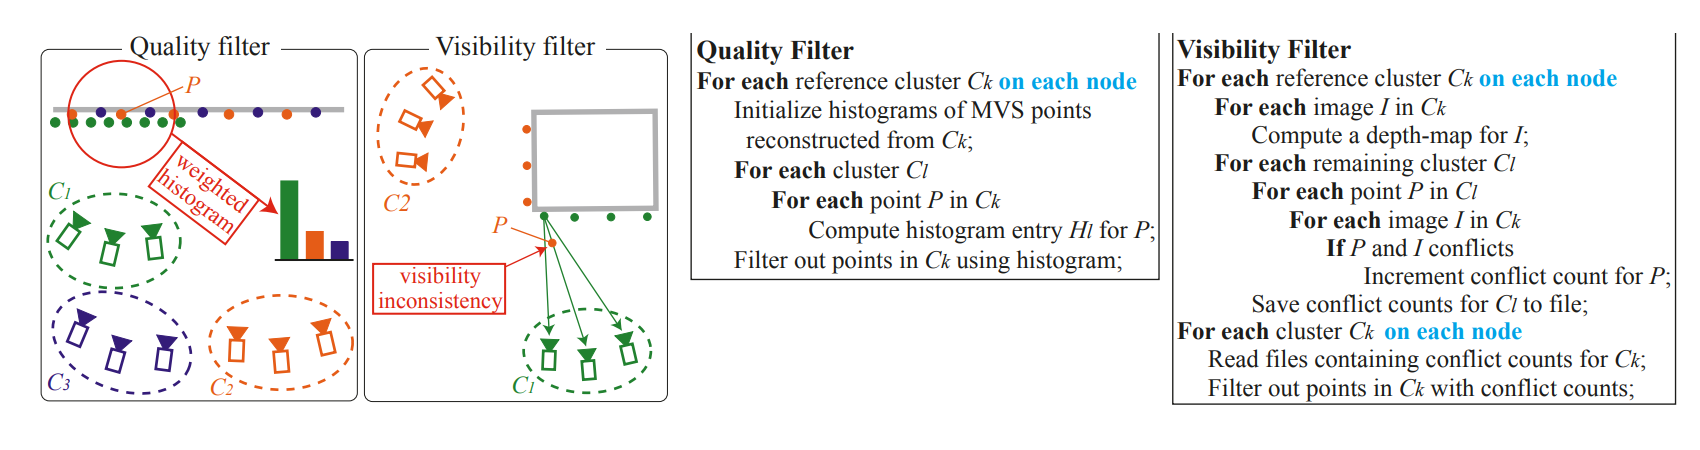
\includegraphics[width=0.5\linewidth]{figs/filtropmvs.png}
	\caption{%
	Usabilidade dos filtros de qualidade e visibilidade, onde são aplicados fora do núcleo, assim como em paralelo. À esquerda, um ponto MVS $P$ é testado usando os filtros. À direita, temos pseudo-códigos, onde os \emph{loops} destacados em azul podem ser executados em paralelo.
	\cite{furukawa2010towards}.
	}\label{fig:filtropmvs}
\end{figure} 

\subsubsection{Filtro de Qualidade}

A mesma região de superfície pode ser reconstruída em múltiplos clusters com qualidade de reconstrução variável: grupos próximos produzem pontos densos e precisos, enquanto cachos distantes produzem pontos escassos e ruidosos. Queremos filtrar o último, que é realizado pelo seguinte filtro de qualidade. Assumimos que $P_j$ e $V_j$ denotarem um ponto MVS e suas informações de visibilidade estimadas pelo algoritmo MVS, respectivamente. Supomos que $P_j$ foi reconstruído a partir do \emph{cluster} $C_k$. Primeiramente coletamos pontos MVS ${Q_m}$ e sua informação de visibilidade ${V_m}$ de todos os \emph{clusters} que possuam normais compatíveis com $P_j$, isto é, a diferença de ângulo menores que $90^\circ$ e seus locais projetados estejam dentro de $n$ pixels de $P_j$ em cada imagem em $V_j$, (no caso, experimentalmente, $n=8$). A partir dos pontos MVS obtidos, calculamos um histograma ($H_l$), onde $H_l$ é a soma da acurácia das precisões $f(Q_m,V_m)$ associadas a pontos MVS reconstruídos a partir de $C_l$. Uma vez que um \emph{cluster} possua pontos acurados e densos, este deverá ter um valor significativamente maior do que os outros. $P_j$ é filtrado se o valor do histograma $H_k$ correspondente for inferior a metade do máximo: $Hk < 0,5 max_l H_l$. Repetimos este procedimento examinando cada \emph{cluster} de referência, que pode ser executado em paralelo. 

\subsubsection{Filtro de Visibilidade}

O filtro de visibilidade reforça a consistência das informações de visibilidade associadas aos pontos MVS durante toda a reconstrução. O filtro é, de fato, muito semelhante ao usado no PMVS [7, 9]. A diferença é que o PMVS reforça a consistência intra-cluster dentro de cada cluster, enquanto nosso filtro reforça a consistência de visibilidade inter-cluster em uma reconstrução inteira comparando as saídas PMVS de todos os clusters. Mais concretamente, para cada ponto MVS, contamos o número de vezes que ele conflita com reconstruções de outros clusters. O ponto é eliminado se a contagem de conflitos~\cite{furukawa2010towards,furukawa2010accurate} for superior a três.

\end{itemize}
% =================================================================

